% Digital Logic Report Template
% Created: 2020-01-10, John Miller

%==========================================================
%=========== Document Setup  ==============================

% Formatting defined by class file
\documentclass[11pt]{article}

% ---- Document formatting ----
\usepackage[margin=1in]{geometry}	% Narrower margins
\usepackage{booktabs}				% Nice formatting of tables
\usepackage{graphicx}				% Ability to include graphics
\usepackage[section]{placeins}      % Stops floats from happening

%\setlength\parindent{0pt}	% Do not indent first line of paragraphs 
\usepackage[parfill]{parskip}		% Line space b/w paragraphs
%	parfill option prevents last line of pgrph from being fully justified

% Parskip package adds too much space around titles, fix with this
\RequirePackage{titlesec}
\titlespacing\section{0pt}{8pt plus 4pt minus 2pt}{3pt plus 2pt minus 2pt}
\titlespacing\subsection{0pt}{4pt plus 4pt minus 2pt}{-2pt plus 2pt minus 2pt}
\titlespacing\subsubsection{0pt}{2pt plus 4pt minus 2pt}{-6pt plus 2pt minus 2pt}

% ---- Hyperlinks ----
\usepackage[colorlinks=true,urlcolor=blue]{hyperref}	% For URL's. Automatically links internal references.

% ---- Code listings ----
\usepackage{listings} 					% Nice code layout and inclusion
\usepackage[usenames,dvipsnames]{xcolor}	% Colors (needs to be defined before using colors)

% Define custom colors for listings
\definecolor{listinggray}{gray}{0.98}		% Listings background color
\definecolor{rulegray}{gray}{0.7}			% Listings rule/frame color

% Style for Verilog
\lstdefinestyle{Verilog}{
	language=Verilog,					% Verilog
	backgroundcolor=\color{listinggray},	% light gray background
	rulecolor=\color{blue}, 			% blue frame lines
	frame=tb,							% lines above & below
	linewidth=\columnwidth, 			% set line width
	basicstyle=\small\ttfamily,	% basic font style that is used for the code	
	breaklines=true, 					% allow breaking across columns/pages
	tabsize=3,							% set tab size
	commentstyle=\color{gray},	% comments in italic 
	stringstyle=\upshape,				% strings are printed in normal font
	showspaces=false,					% don't underscore spaces
}

% How to use: \Verilog[listing_options]{file}
\newcommand{\Verilog}[2][]{%
	\lstinputlisting[style=Verilog,#1]{#2}
}




%======================================================
%=========== Body  ====================================
\begin{document}

\title{ELC 2137 Lab 07: Binary Coded Decimal}
\author{Maddie Vorhies}

\maketitle


\section*{Summary}

The goal of this lab was to implement a 7-segment display, with binary as the input and hex as the output. To do this, I started out by using the double-dabble algorithm to convert hex values to BCD. I then drew the picture for an 11-bit double-dabble circuit and built it. I then created a simulation to test the circuit to make sure that it was properly built. I then took the mux and the 7-segment decoder from Lab 06 and modified it to fit into this lab. Then I created the sseg1 that connected all of those together. Lastly, I created a wrapper to make the circuit appear cleaner and more organized. I then hooked up my board to test out my completed circuit. Overall, I was able to successfully build the circuit and have it display the proper values on the board.


\section*{Results}

\begin{figure}[ht]\centering
	\begin{tabular}[ht]{c|c|c}
		Time (ns) & Input & Output\\
		\midrule
		0 & 0000 & 0000\\
		10 & 0001 & 0001\\
		20 & 0010 & 0010\\
		30 & 0011 & 0011\\
		40 & 0100 & 0100\\
		50 & 0101 & 1000\\
		60 & 0110 & 1001\\
		70 & 0111 & 1010\\
		80 & 1000 & 1011\\
		90 & 1001 & 1100\\
		100 & 1010 & 1101\\
		110 & 1011 & 11100\\
		120 & 1100 & 1111\\
		130 & 1101 & 0000\\
		140 & 1110 & 0001\\
		150 & 1111 & 0010\\
		\bottomrule
	\end{tabular}\medskip
	
	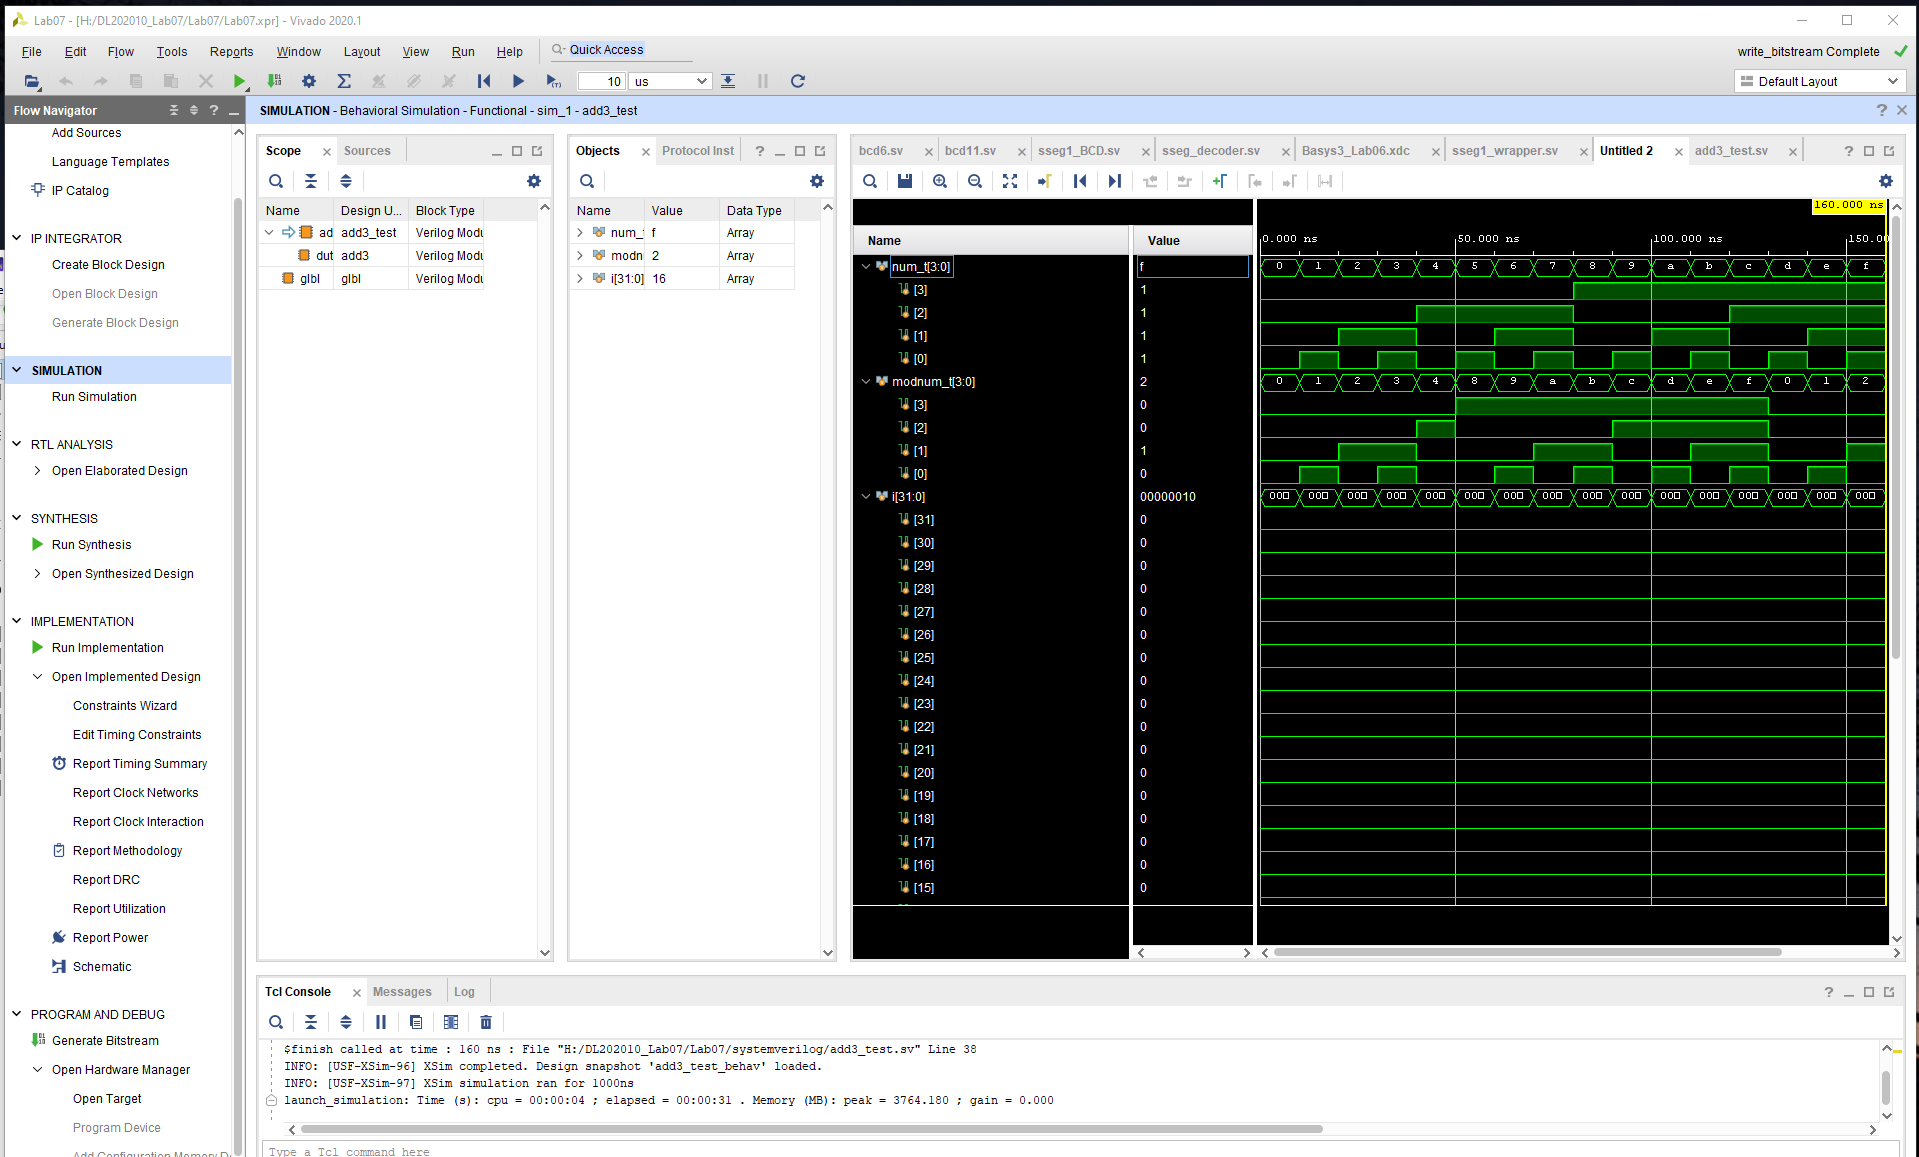
\includegraphics [width=1.0\textwidth,trim=640 475 10 135, clip]{Add3_sim}
	\caption{Simulation Waveform and ERT of Add3}
	\label{fig:sim_with_table}
\end{figure}
	
	\begin{figure}[ht]\centering
		\begin{tabular}[ht]{c|c|c|c}
			Time (ns) & Input & Ouput & decimal\\
			\midrule
			0 & 100100 & 00110110 & 36\\
			10 & 001101 & 00010011 & 13\\
			20 & 111001 & 01010111 & 57\\
			\bottomrule
		\end{tabular}\medskip
		
		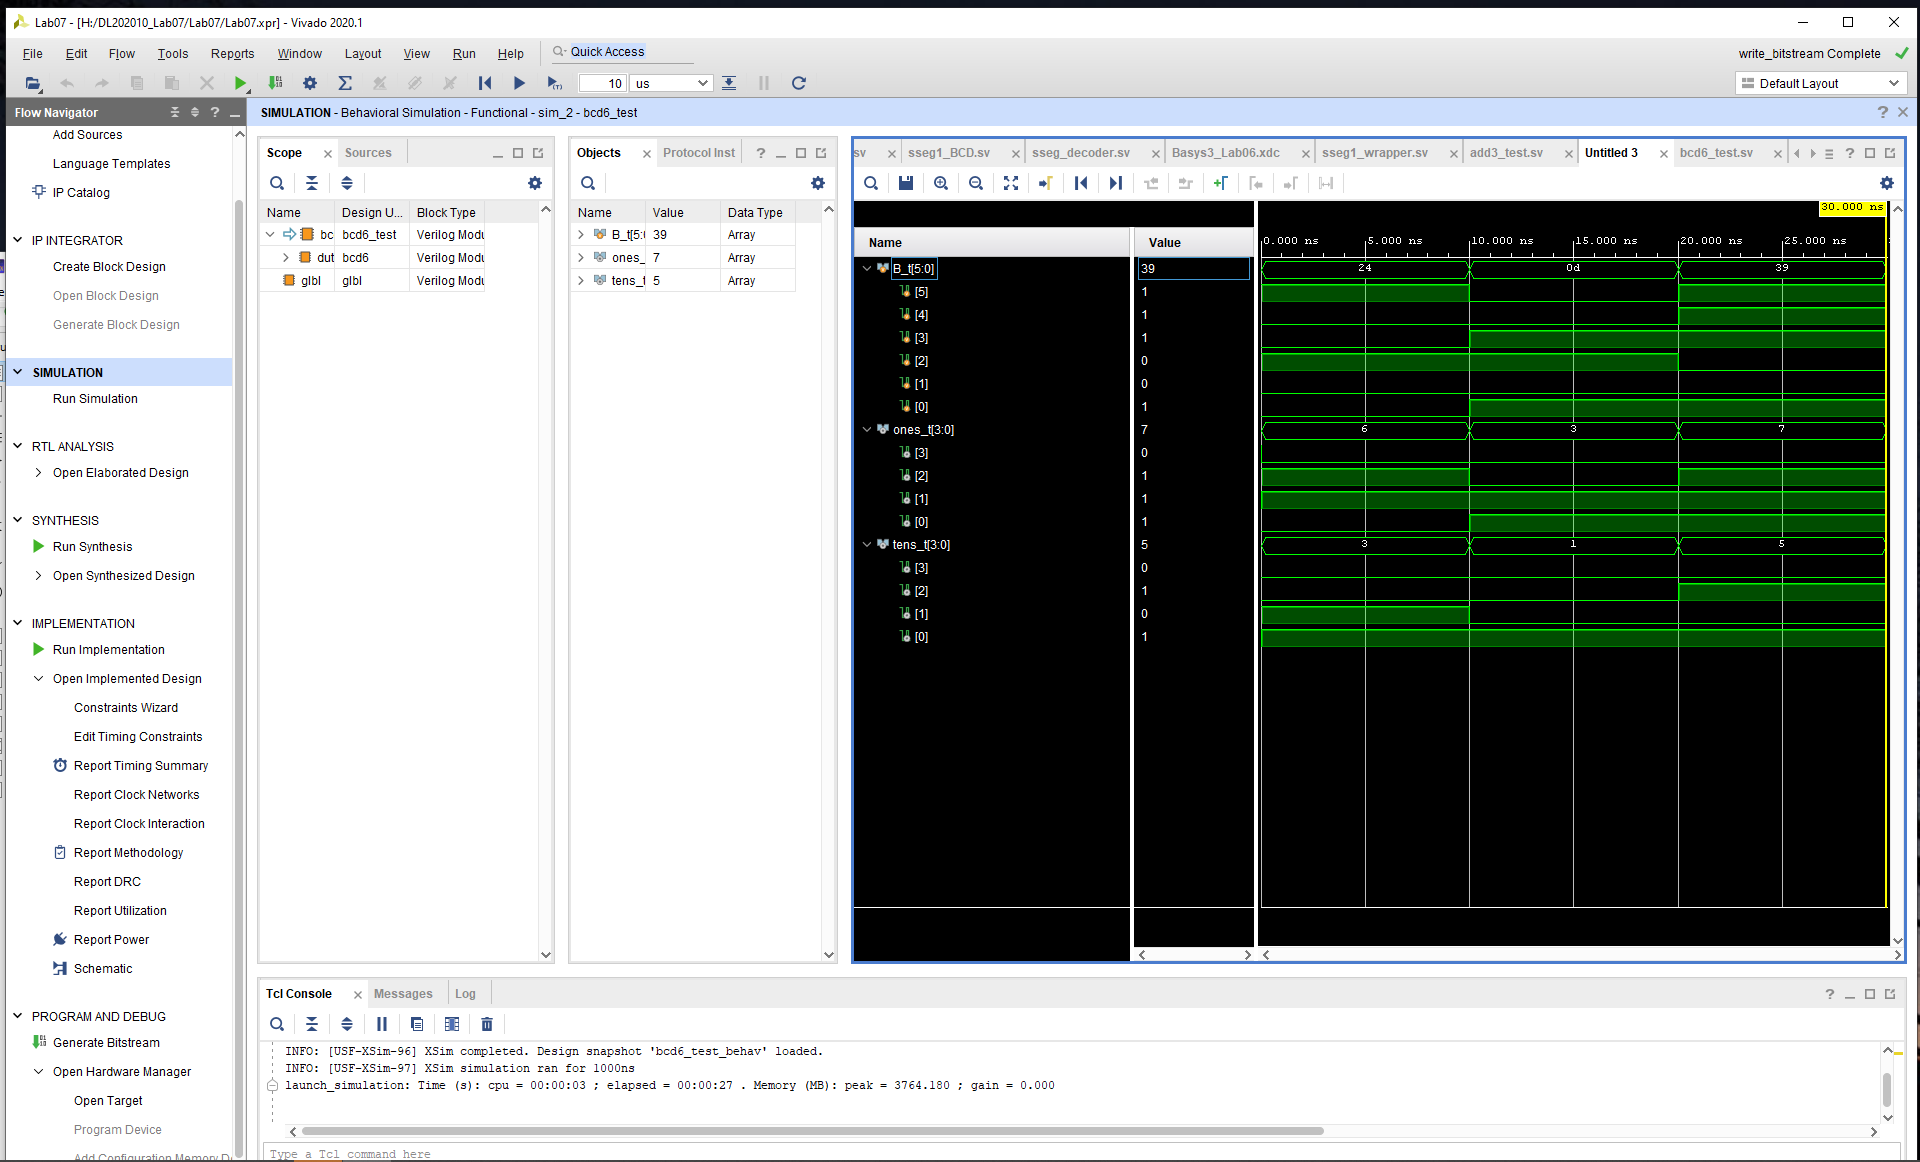
\includegraphics [width=1.0\textwidth,trim=640 450 10 135, clip]{bcd6_sim}
		\caption{Simulation Waveform and ERT of 6-bit double dabble circuit}
		\label{fig:sim_with_table}
		
	\end{figure}

	\begin{figure}[ht]\centering
	\begin{tabular}[ht]{c|c|c|c}
		Time (ns) & Input & Ouput & decimal\\
		\midrule
		0 & 10010011101 & 0001000110000001 & 1181\\
		10 & 00110110110 & 0000010000111000 & 438\\
		20 & 11100110001 & 0001100001000001 & 1841\\
		\bottomrule
	\end{tabular}\medskip
	
	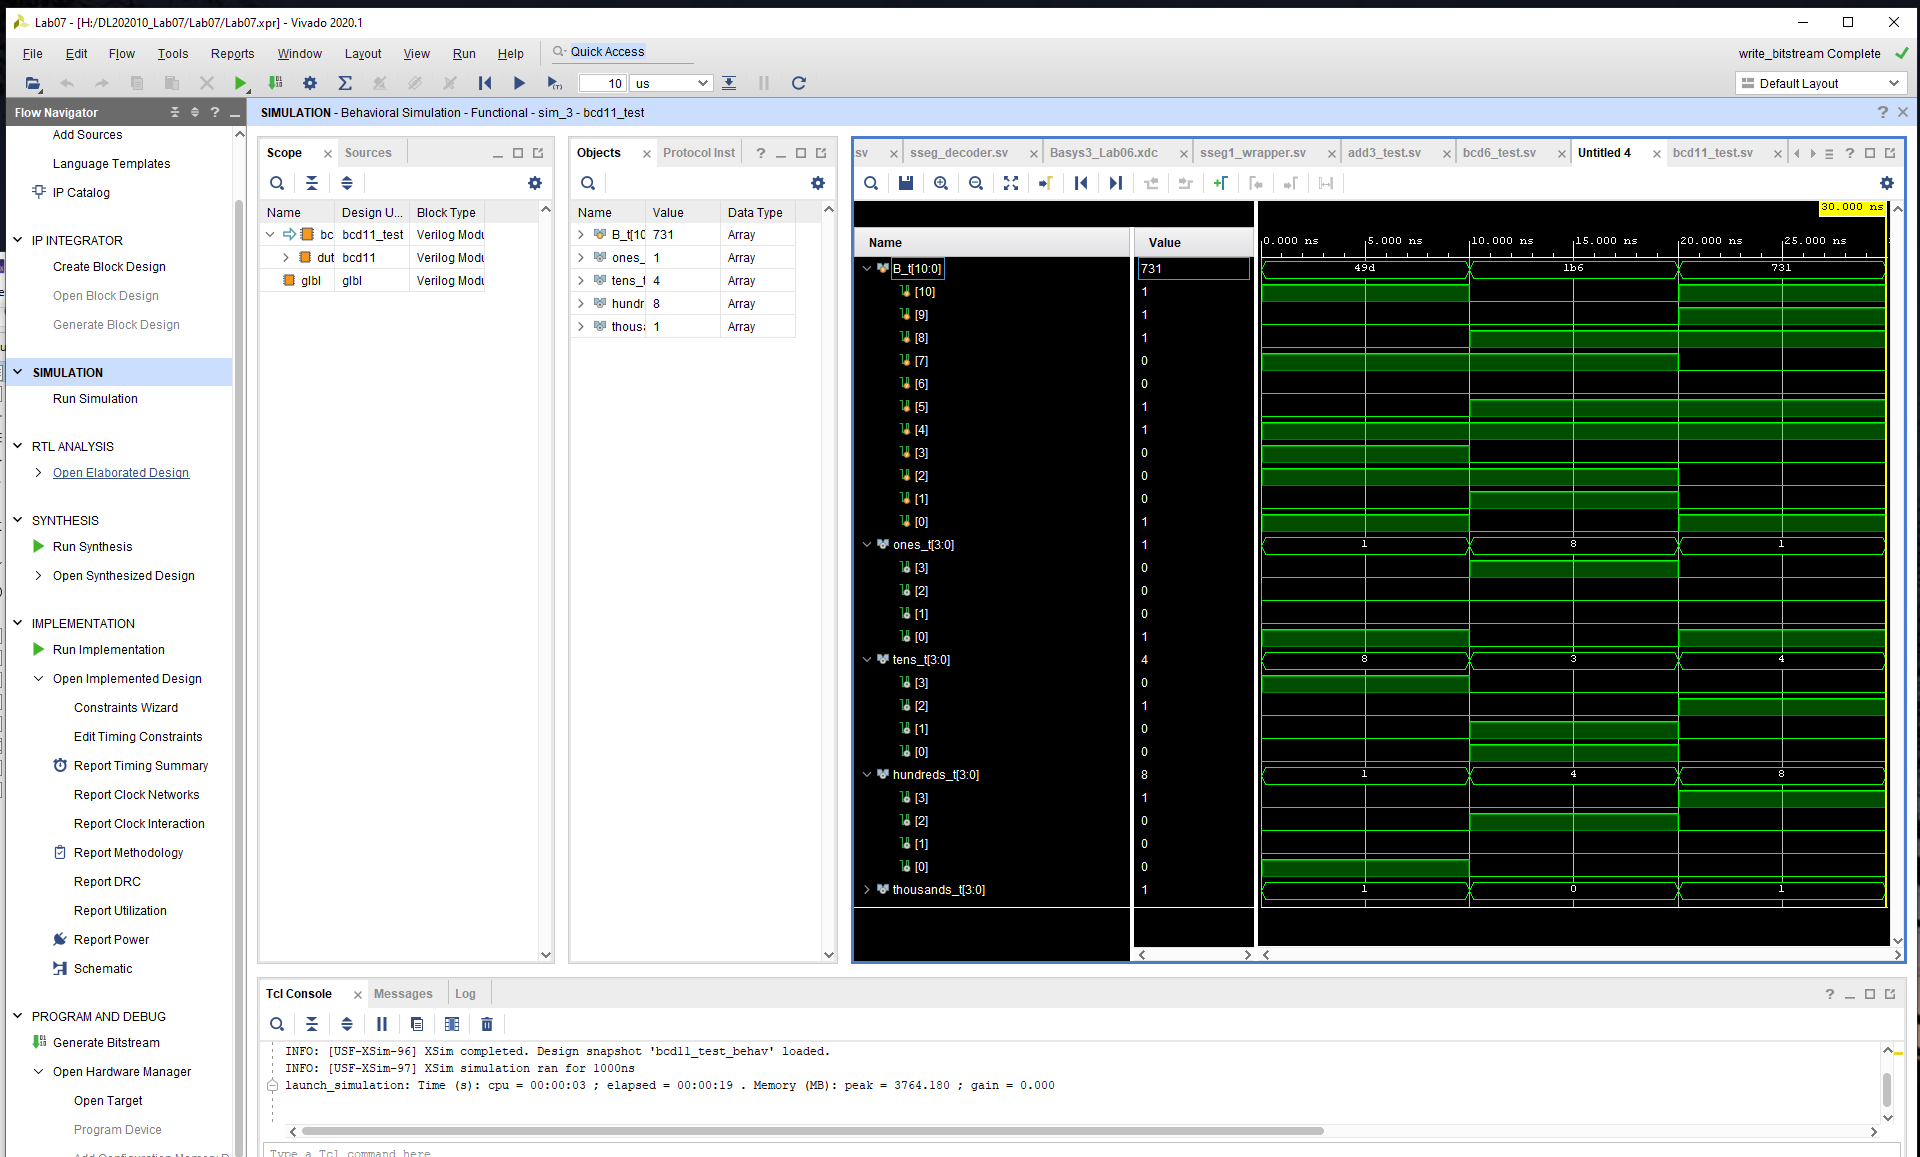
\includegraphics [width=1.0\textwidth,trim=640 275 10 135, clip]{bdc11_sim}
	\caption{Simulation Waveform and ERT of 11-bit double dabble circuit}
	\label{fig:sim_with_table}
	
\end{figure}

\begin{figure}[ht]\centering
	\caption{11-bit double dabble circuit drawing}
	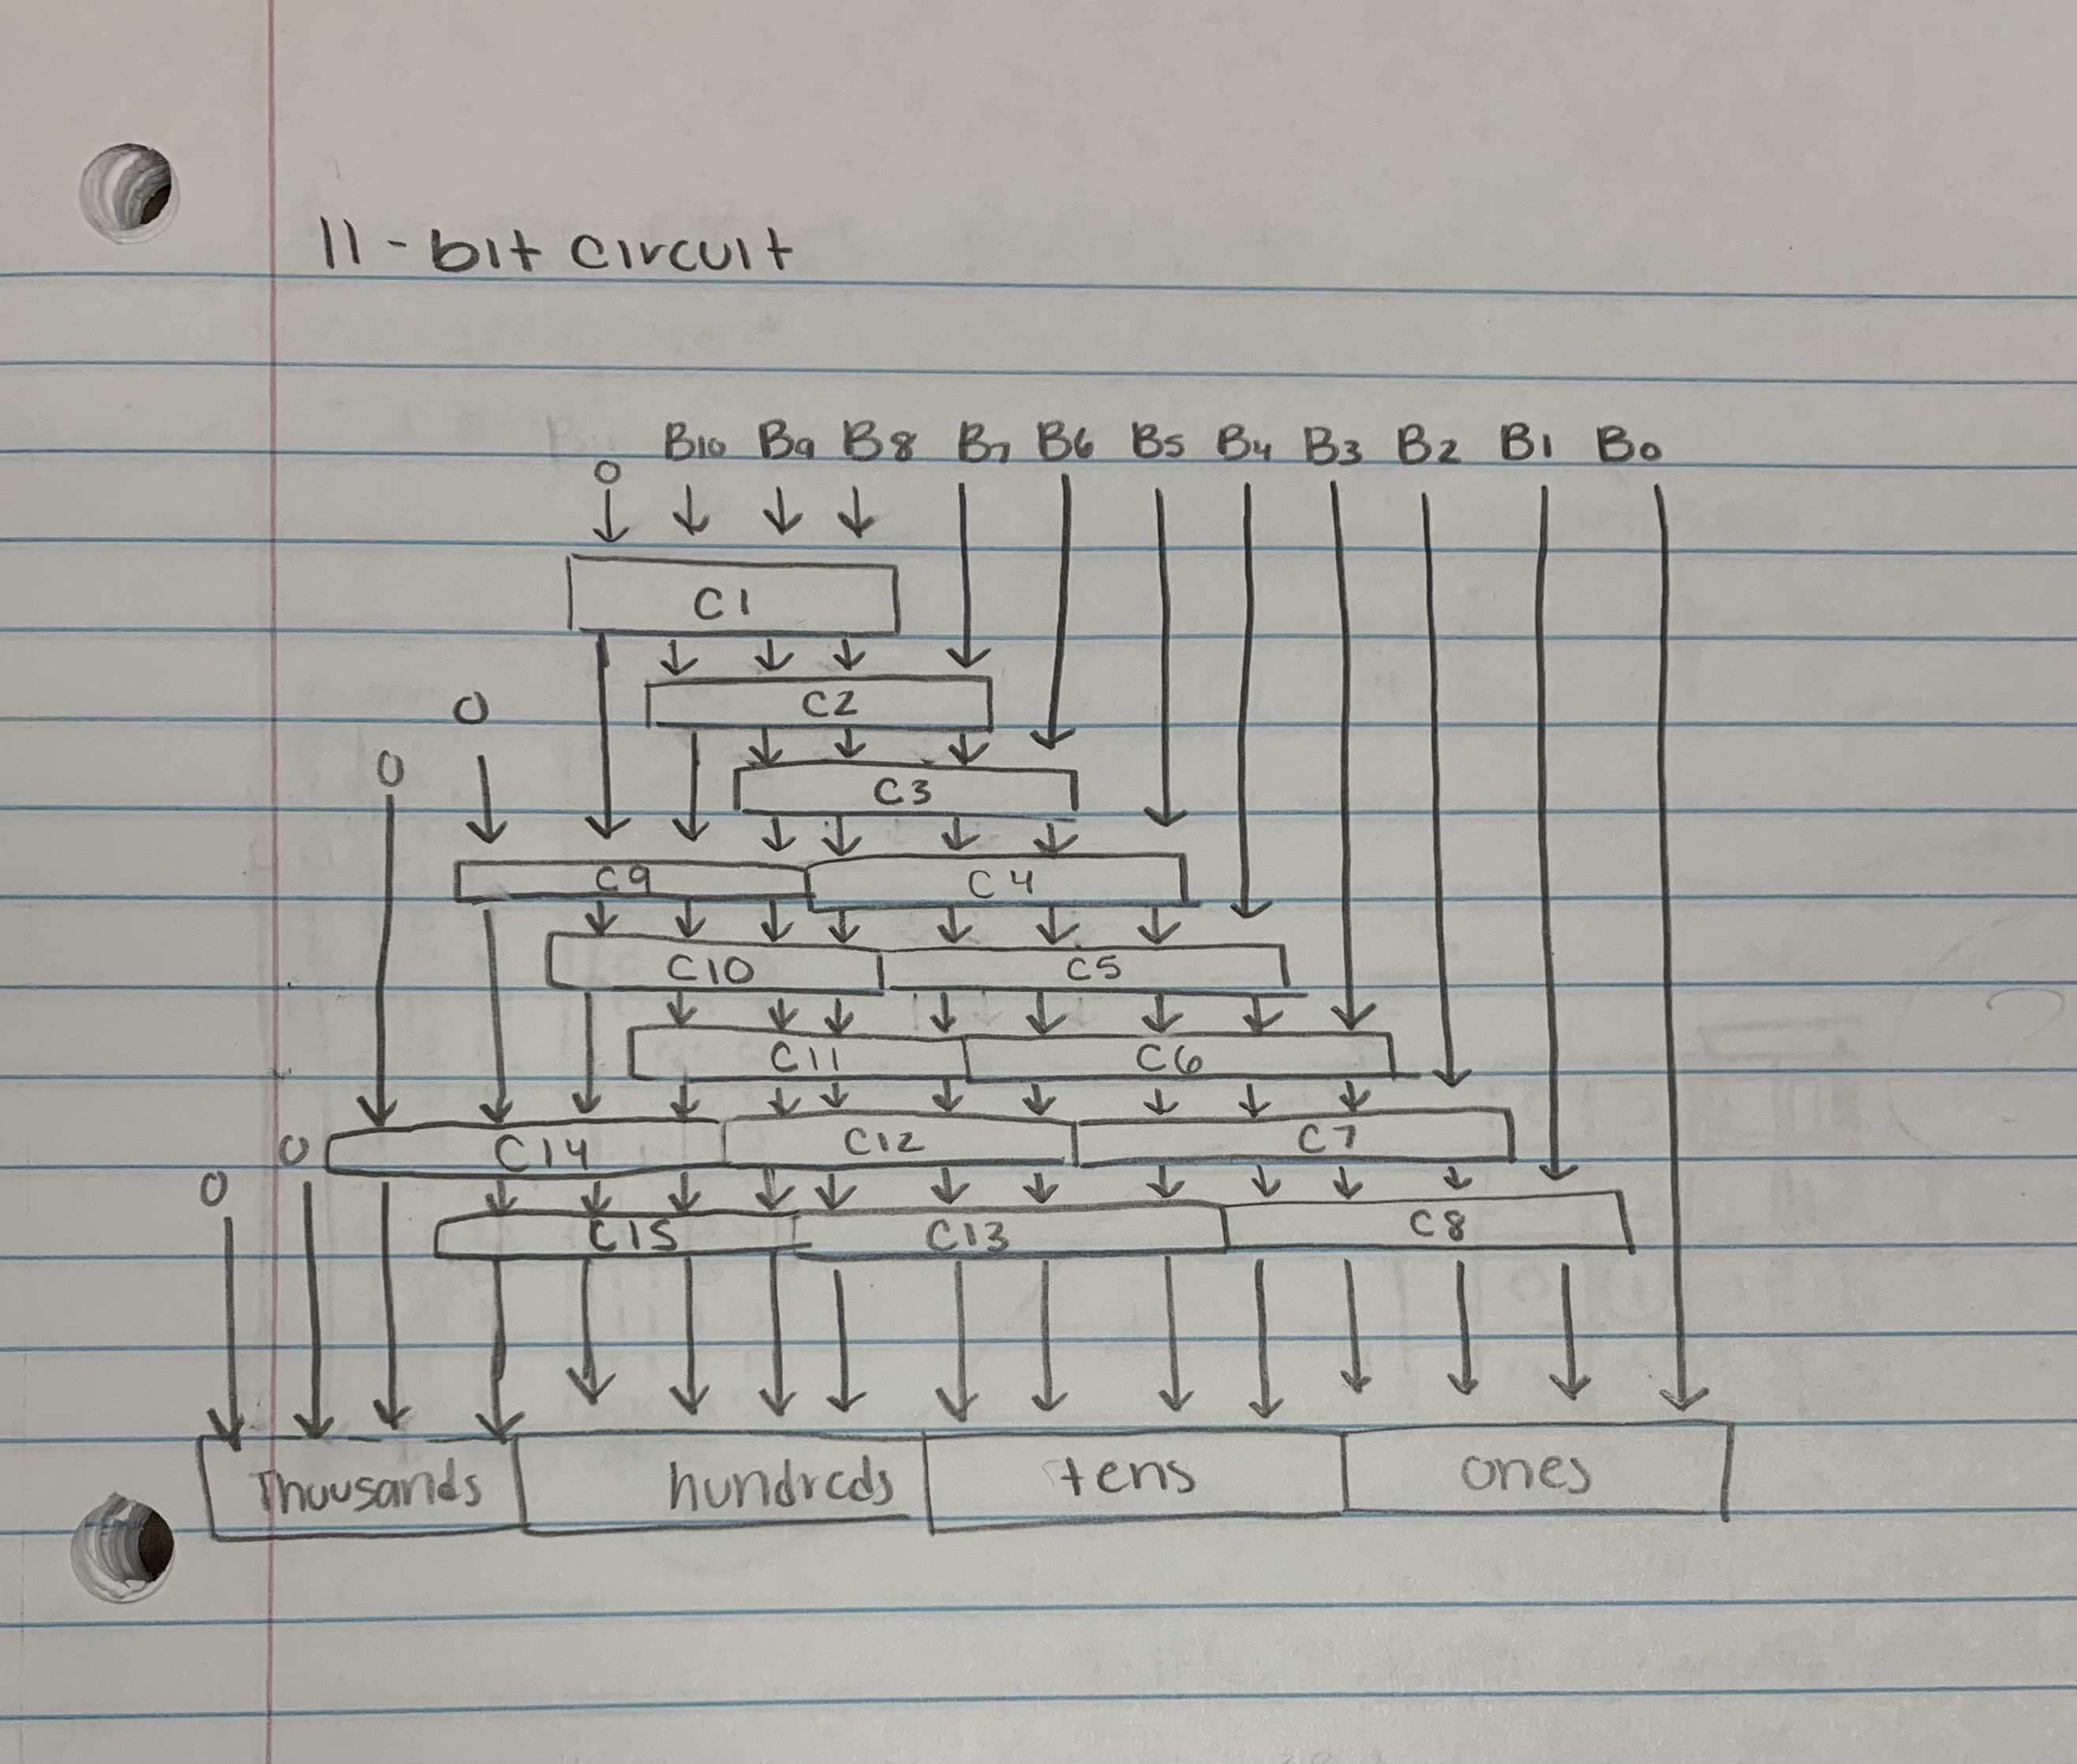
\includegraphics [width=1\textwidth,trim=0 0 0 0, clip]{11bit_circuit}
\end{figure}

\begin{table}[h]\centering
	\begin{tabular}{cc}
		First Digit & Second Digit \\
		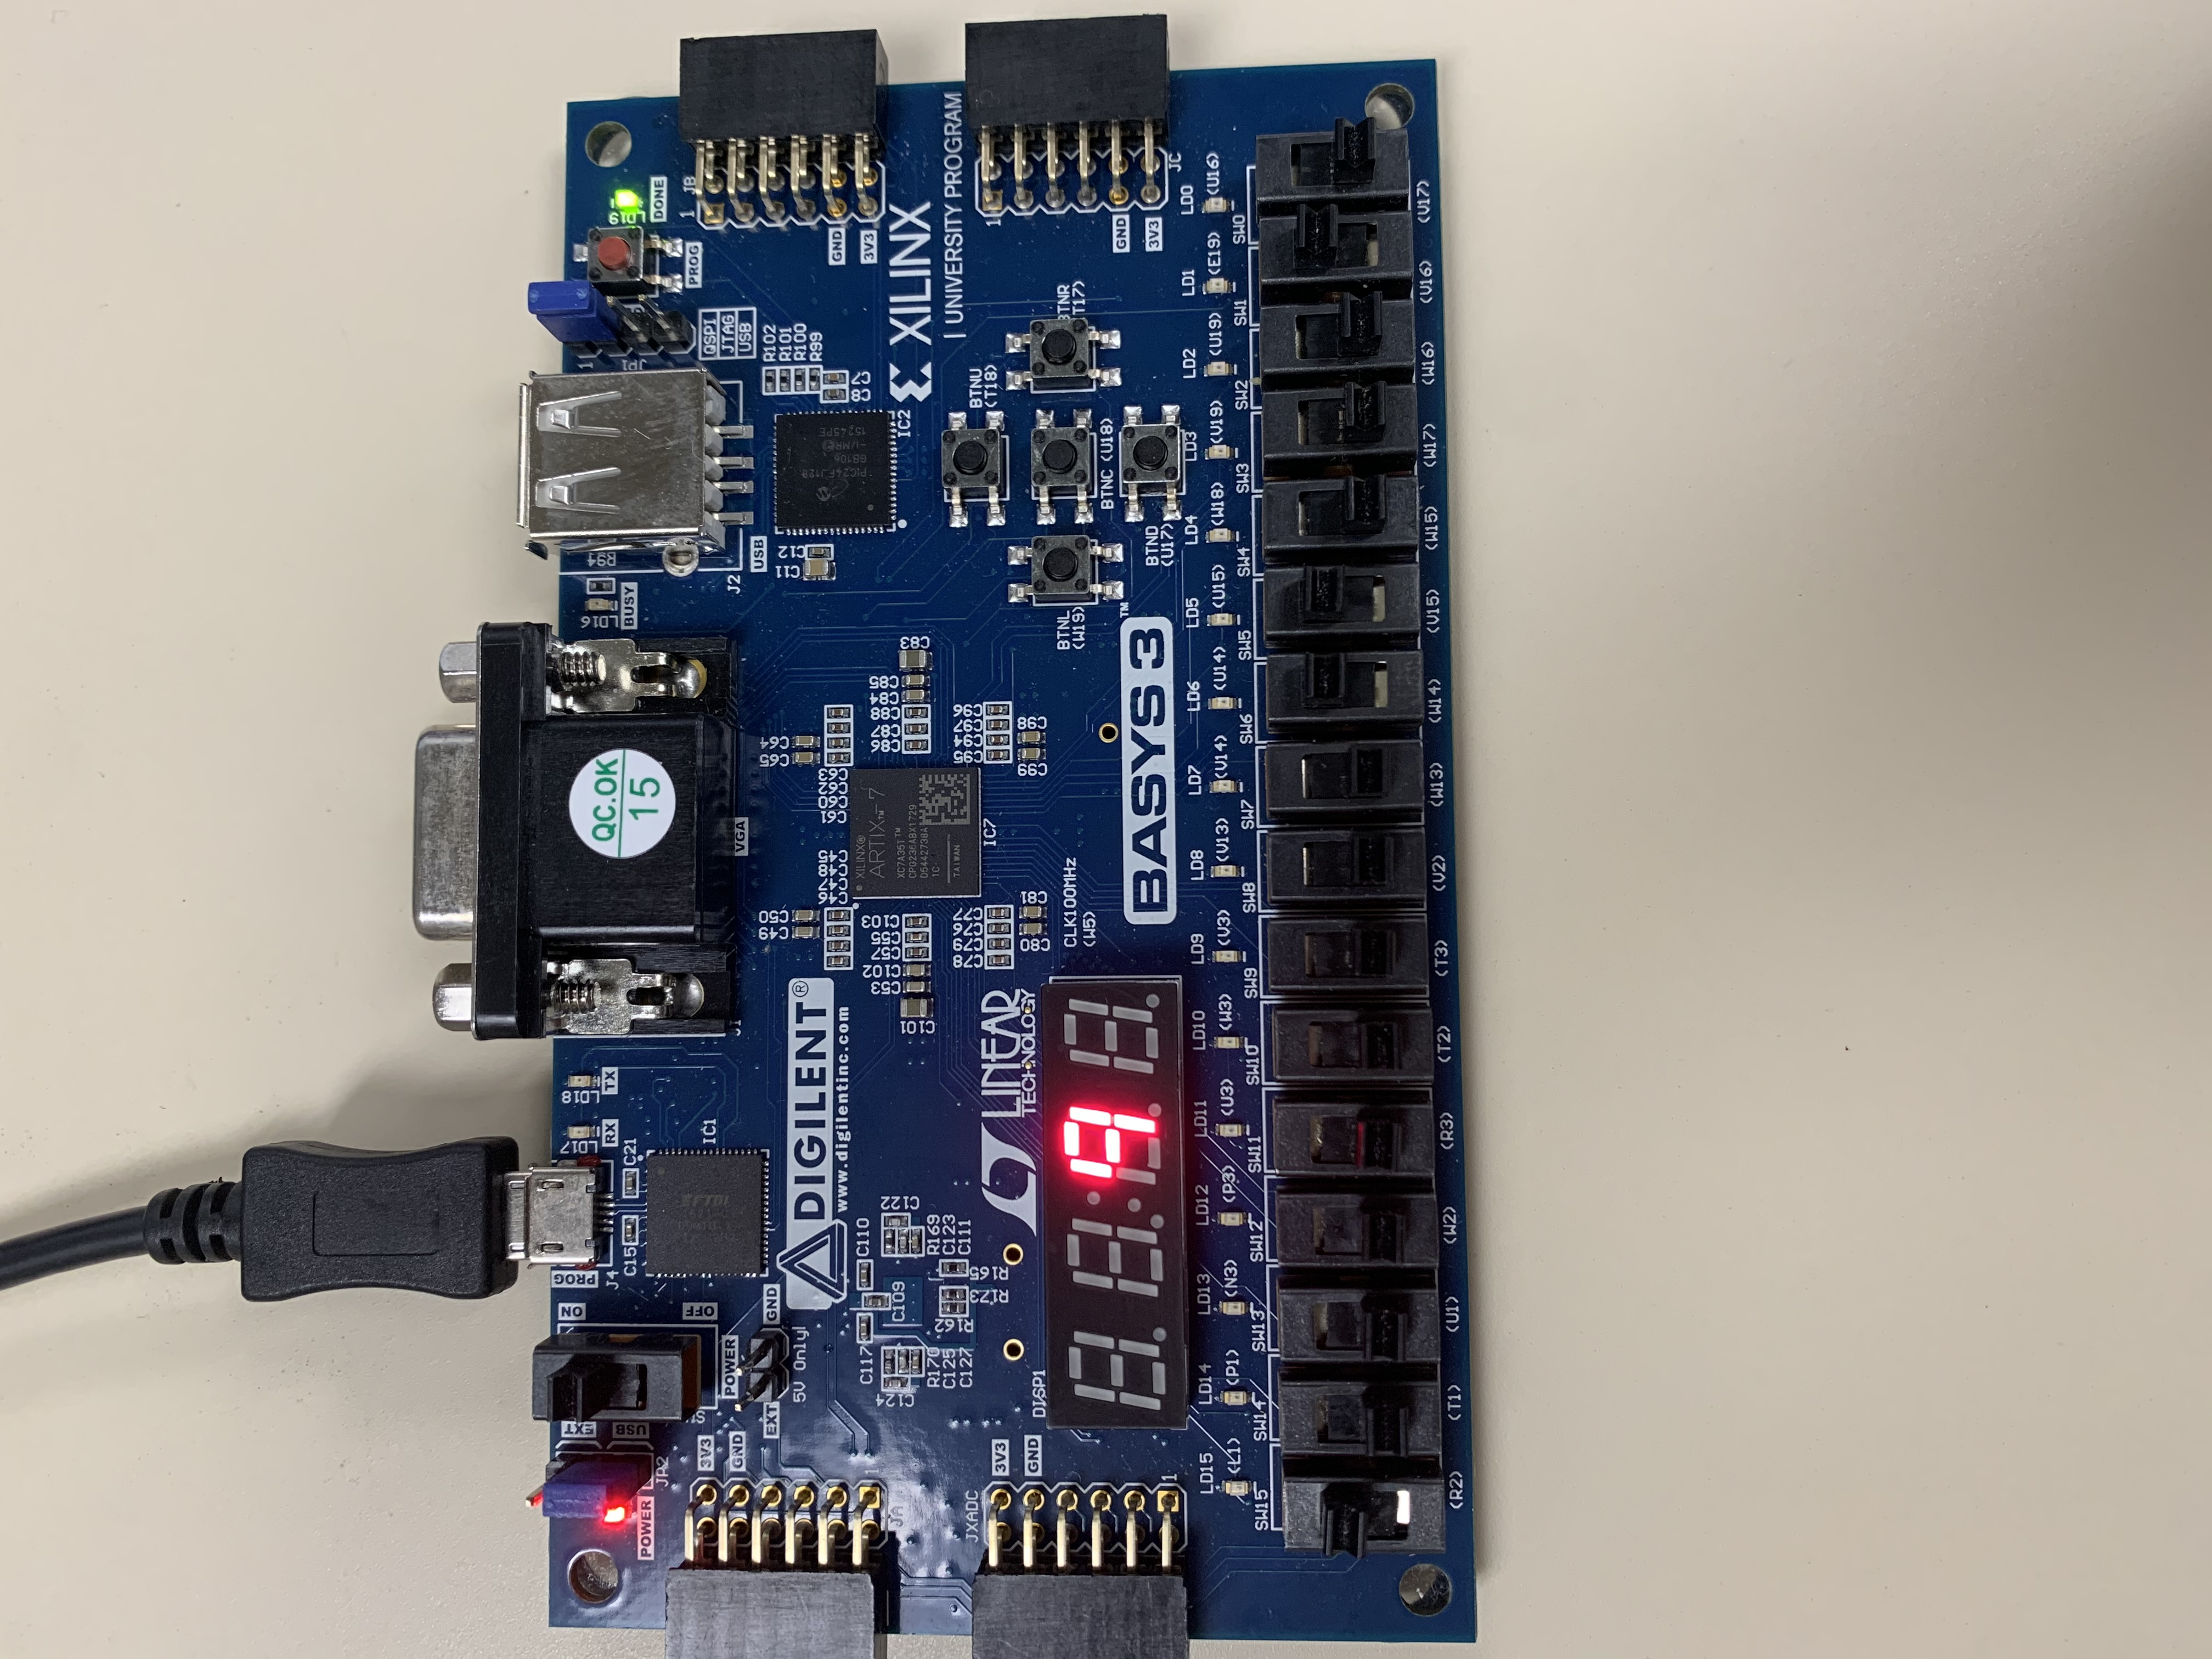
\includegraphics [width=0.5\textwidth,trim=0 0 0 0, clip, angle = 270]{Basys3_pic9} &
		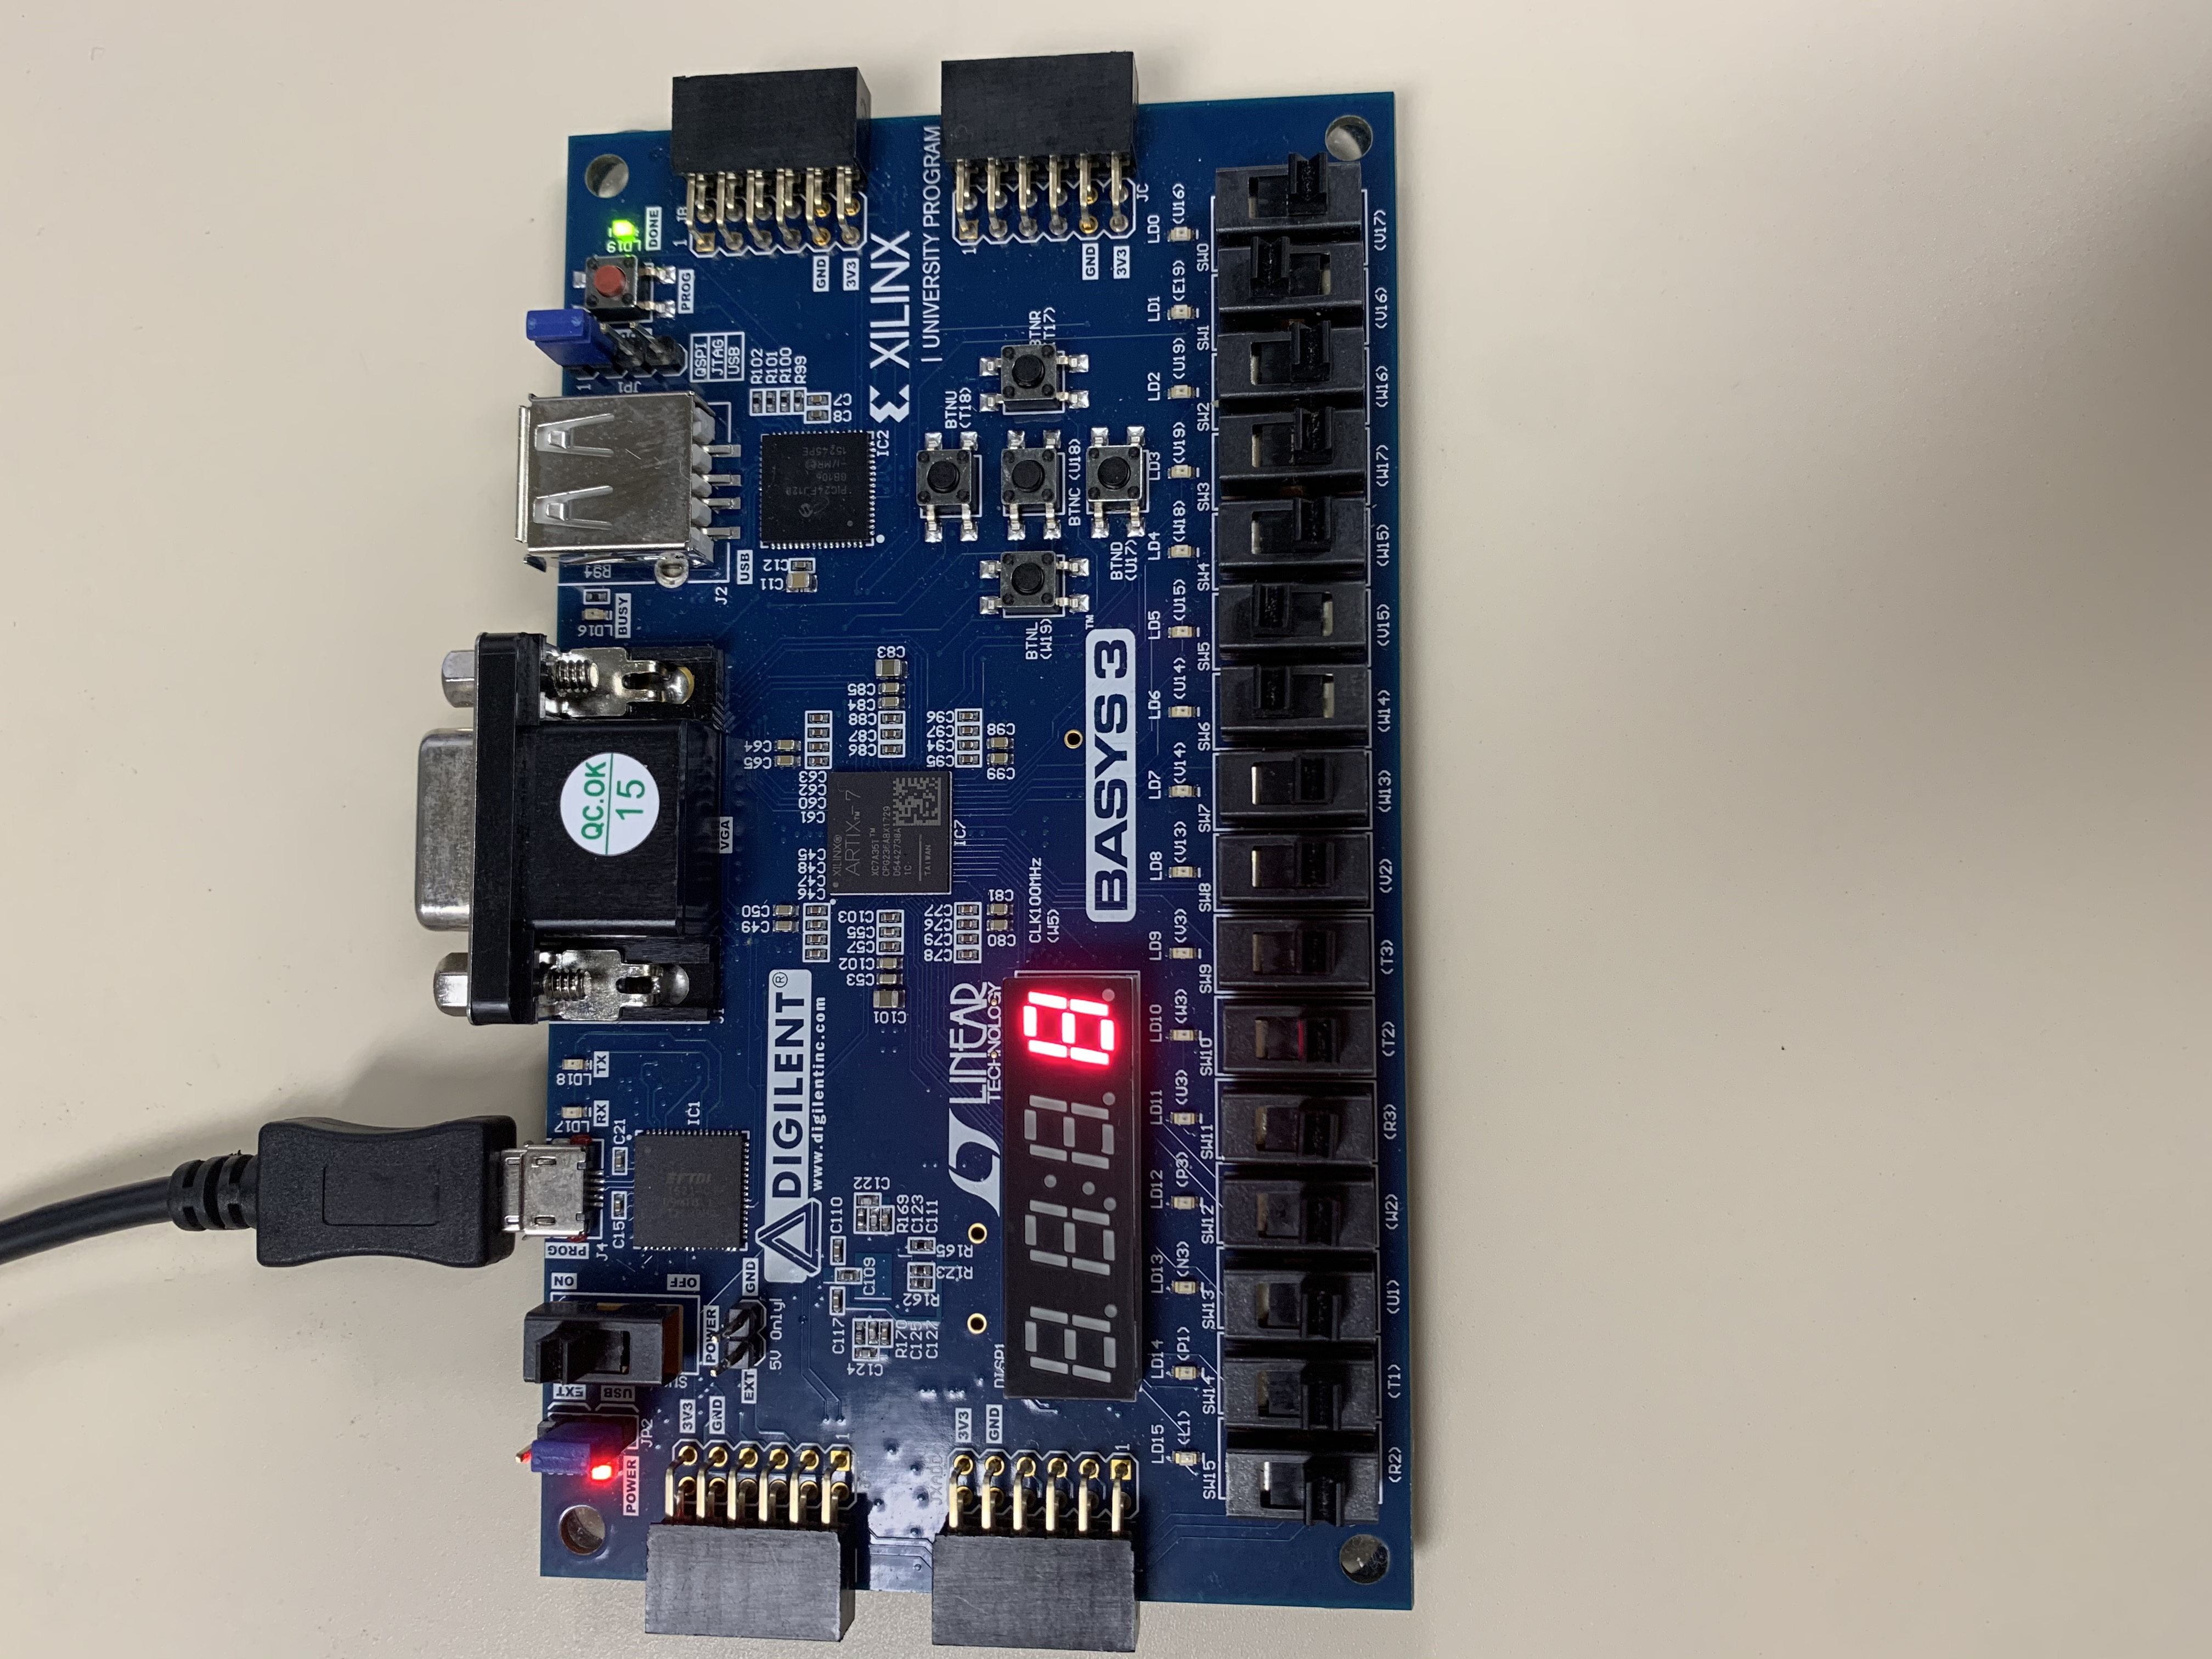
\includegraphics [width=0.5\textwidth,trim=0 0 0 0, clip, angle = 270]{Basys3_pic8} \\
	\end{tabular}
	\caption{Board Pictures}
	\label{fig:sim_with_table}
\end{table}

\section*{Code}

\Verilog{Lab07/systemverilog/add3.sv}

\Verilog{Lab07/systemverilog/add3_test.sv}

\Verilog{Lab07/systemverilog/bcd6.sv}

\Verilog{Lab07/systemverilog/bcd6_test.sv}

\Verilog{Lab07/systemverilog/bcd11.sv}

\Verilog{Lab07/systemverilog/bcd11_test.sv}

\Verilog{Lab07/systemverilog/sseg1_BCD.sv}

\Verilog{Lab07/systemverilog/sseg1_wrapper.sv}


\end{document}
